\section{Project management}
\label{section:project_management}

We will discuss in this section everything concerning the management of the project: \textit{scope}, \textit{schedule} and \textit{budget}. However, we must stress that this classical approach of management analysis is not really suited for our needs. Instead, a more \textit{Agile}\footnote{Agile software development is based on the \textit{Agile manifesto}~\cite{website:AgileManifesto}.} methodology will be applied. We cover this on the Methodology section, but there is an important conceptual change to be taken into account: the different driving force of the project. Whereas in classical project management the scope-schedule-budget triad is what must be controlled, in an Agile project management approach it is \textit{value}. Indeed, \textit{quality} must be ensured so maximum value is delivered to the project's stakeholders, thus being scope, cost and schedule constraints to these primary goals.

\begin{figure}[h]
	\centering
	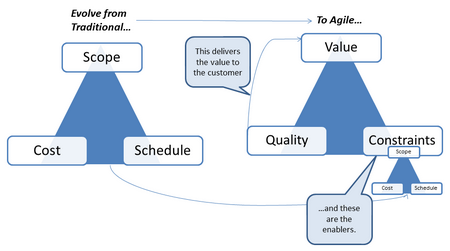
\includegraphics[width=0.7\linewidth]{figures/agiletriangle-1.png}
	\caption{Traditional to Agile project management evolution. Source:~\cite{website:AgileTriangle}}
	\label{fig:agile-pm}
\end{figure}

\subsection{Scope}
\label{section:scope}

One of the first things to do, when beginning any project is delimiting its scope, this is, deciding \textit{what} will be done and \textit{how}, in terms of resources and methodology, for example.

\subsubsection{Requirement analysis}

We already stated in section~\ref{section:introductionNutshell} what the main goal of this project is. A more detailed list of the project's requirements is the following one:

\begin{itemize}
	\item \textbf{Functional requirements:} 
	\begin{enumerate}
		\item Implement privacy preserving stream mining \textit{filters}\footnote{Within the MOA context, \textit{filters} are procedures applied to data prior to their analysis using machine learning algorithms.} for the MOA stream mining framework. The suggested algorithms to be implemented are:
		\begin{enumerate}
			\item Noise addition~\cite[p.~54]{book:StatisticalDisclosureControl}
			\item Multiplicative noise~\cite[p.~57]{book:StatisticalDisclosureControl}
			\item Microaggregation~\cite[p.~60]{book:StatisticalDisclosureControl}
			\item Rank shuffling~\cite[p.~73]{book:StatisticalDisclosureControl}
			\item Differential privacy~\cite{Dwork06differentialprivacy}
		\end{enumerate}
	\end{enumerate}
	
	\item \textbf{Non-functional requirements:}
	\begin{enumerate}
		\item \textbf{Correctness:} privacy protection is at stake in this project, so algorithms must be implemented correctly, from the theoretical point of view, in order to not ease information disclosure when they are used.
		\item \textbf{Efficiency:} given that no data mining process can scale well if its algorithms are slow, effort will be put in making them the most efficient we can.
		\item \textbf{Test coverage:} measures and tests will be performed to assess the quality of the developed software, as well as its scalability and performance, which is paramount in this project’s context.
		\item \textbf{Documentation:} MOA is an \textit{open source} data mining framework, which means that its community can assess how is it built and how to improve it. One of the benefits of the open source development model is that software can be safer, more robust and efficient, by receiving contributions from different developers. If people are to continue improving the work done, it has to be well documented.
	\end{enumerate}
\end{itemize}

\subsubsection{Scope risks analysis}

The methodology approach used in this project will be based on Agile principles. This involves several decisions on how to manage the project and its requirements.\\

In this particular project, if we are to examine the classic constraints that we talked about at the beginning of this section, we do know that the schedule is fixed (perhaps not the planning, but the final milestone) and this forces us to let the scope opened. This is, we will implement as much features as we can, assessing their quality, but no feature list will be fixed from the beginning of the project.\\

Because we will be working on the basis of an \textit{open scope}, deviations in this field are likely to happen. These, however, will not pose to be a project failure in any case, because it has been agreed to be developed this way.

\subsubsection{Methodology}

Agile methods will be applied throughout the development phase of this project. Some of the key concepts and practices in this respect are:

\begin{itemize}
	\item Short to mid range development \textbf{sprints} (phases), in order to keep track of the project’s evolution and to be able to react to changes, unforeseen constraints or scope drifts.
	\item \textbf{Constant meetings} with the project’s stakeholders, in which the progress and deviations of the project will be assessed. Measures to alleviate them will be taken in these meetings.
	\item Use of \textbf{burndown charts} - graphical representations of work left to do versus time.
\end{itemize}


\subsection{Schedule}
\subsubsection{Overall duration}

Taking a general look at the project’s schedule, we can estimate it to have a total duration of about 5 months. Even though it was registered on July, 2014, the project did not begin until September, because August is the only month I can have holidays, due to job restrictions. Considering the next possible project’s lecture shifts, we believe that the one taking place in December is too close in time. Thus, the project will endure until January the 26th, 2015. This should give us time enough to develop the project and document it without too much pressure, which is key to fulfill one of the main established goals: high quality results.

\subsubsection{Schedule slack}

The project schedule we present herein does not fill up the total amount of time available - more than two weeks are left blank, with no assigned tasks. This is intended because of the following reasons:

\begin{itemize}
	\item The amount of time needed to develop the proposed algorithms is uncertain. It is hard to estimate the time it may take, because I have no previous knowledge on the area. Therefore, we opted for, in one hand, an open scope approach, and, on the other, leaving a considerable time gap between the last planned task and the project’s final milestone: its defense. Being conservative, if the development of any proposed method is delayed, we still have some leeway to introduce schedule changes, without risking the project’s success.
	
	\item We have estimated the project’s report confection and the defense presentation rehearsals to be 35 and 7 days, respectively, but depending on how much development is finally carried out, it might not be time enough to write down the report. Extra time for doing it can be then borrowed from the schedule slack time.
	
\end{itemize}

\subsubsection{Schedule monitoring \& changes}

For the development phase of the project, the most suitable way to monitor the schedule we have found is applying an Agile approach to the process. We will work in one week long sprints, meeting every week to assess the quality of the solutions, the proper progress of the project and to plan what will be done during the following sprint.\\

Sprint planning meetings are where the main goals of the project will be sliced in small tasks, which can be tracked and implemented better, because they are not so complex. Thanks to this constant fine-grained planning process, schedule or scope deviations are detected earlier and can be managed efficiently, reacting before they affect deeper the overall success of the project. Given that no fixed features list is assigned to each sprint of the development phase, if the completion of either of those features is delayed, it can be made to span for some more time.\\

Within each of the development sprints, burn downcharts will be used to monitor the progress of the sprint. These charts are helpful in identifying patterns of work (sprint-end rushes, for example) and can help developers maintain a constant rate of finished features.\\

Besides burn down charts and sprint planning meetings, the use of velocity charts will also be helpful to increase the predictability of the following sprint plannings. The more predictable they are, the less deviations will occur and the schedule will be more likely to be fulfilled.

\subsubsection{Detailed schedule}
\subsection{Budget}